% !TeX program = pdflatex
\documentclass[tikz,border=8pt]{standalone}
\usepackage{tikz}
\usetikzlibrary{calc,positioning}
\definecolor{FigureBlue}{HTML}{2563EB}
\definecolor{FigureOrange}{HTML}{EA580C}
\begin{document}
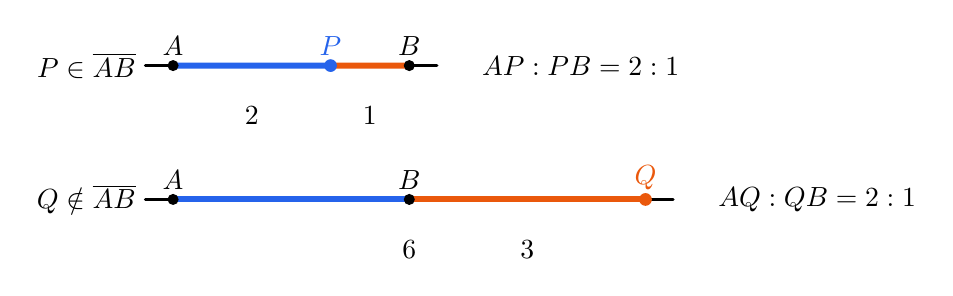
\begin{tikzpicture}[line cap=round,line join=round]
  \coordinate (A) at (0,1.7);
  \coordinate (B) at (3,1.7);
  \pgfmathsetmacro{\internalratio}{2/3}
  \coordinate (P) at ($(A)!\internalratio!(B)$);
  \draw[line width=1.2pt] (-.35,1.7)--(3.35,1.7);
  \draw[FigureBlue,line width=2.2pt] (A)--(P);
  \draw[FigureOrange,line width=2.2pt] (P)--(B);
  \fill (A) circle (2pt) (B) circle (2pt);
  \fill[FigureBlue] (P) circle (2.3pt);
  \node[above] at (A) {$A$};
  \node[above,FigureBlue] at (P) {$P$};
  \node[above] at (B) {$B$};
  \node[left] at (-.35,1.7) {$P\in\overline{AB}$};
  \node[below=4mm] at ($(A)!.5!(P)$) {$2$};
  \node[below=4mm] at ($(P)!.5!(B)$) {$1$};
  \node[right=8mm] at (B) {$AP:PB=2:1$};

  \coordinate (A2) at (0,0);
  \coordinate (B2) at (3,0);
  \coordinate (Q) at ($(A2)!2!(B2)$);
  \draw[line width=1.2pt] (-.35,0)--(6.35,0);
  \draw[FigureBlue,line width=2.2pt] (A2)--(Q);
  \draw[FigureOrange,line width=2.2pt] (B2)--(Q);
  \fill (A2) circle (2pt) (B2) circle (2pt);
  \fill[FigureOrange] (Q) circle (2.3pt);
  \node[above] at (A2) {$A$};
  \node[above] at (B2) {$B$};
  \node[above,FigureOrange] at (Q) {$Q$};
  \node[left] at (-.35,0) {$Q\notin\overline{AB}$};
  \node[below=4mm] at ($(A2)!.5!(Q)$) {$6$};
  \node[below=4mm] at ($(B2)!.5!(Q)$) {$3$};
  \node[right=8mm] at (Q) {$AQ:QB=2:1$};
\end{tikzpicture}
\end{document}
